\documentclass[12pt, A4paper, landscape]{article}
\usepackage[utf8]{inputenc}
\usepackage[left=1cm,right=1cm,top=1cm,bottom=1cm]{geometry}
\usepackage{tikz}

\newcommand{\servidor}[1]{\begin{tabular}{l}
  Servidor: \\
  IP primário: #1
\end{tabular}}
\newcommand{\ipspot}[2]{\begin{tabular}{l}
  IP primário: #1 \\
  IP secundário: #2
\end{tabular}}
\begin{document}
\begin{center}
  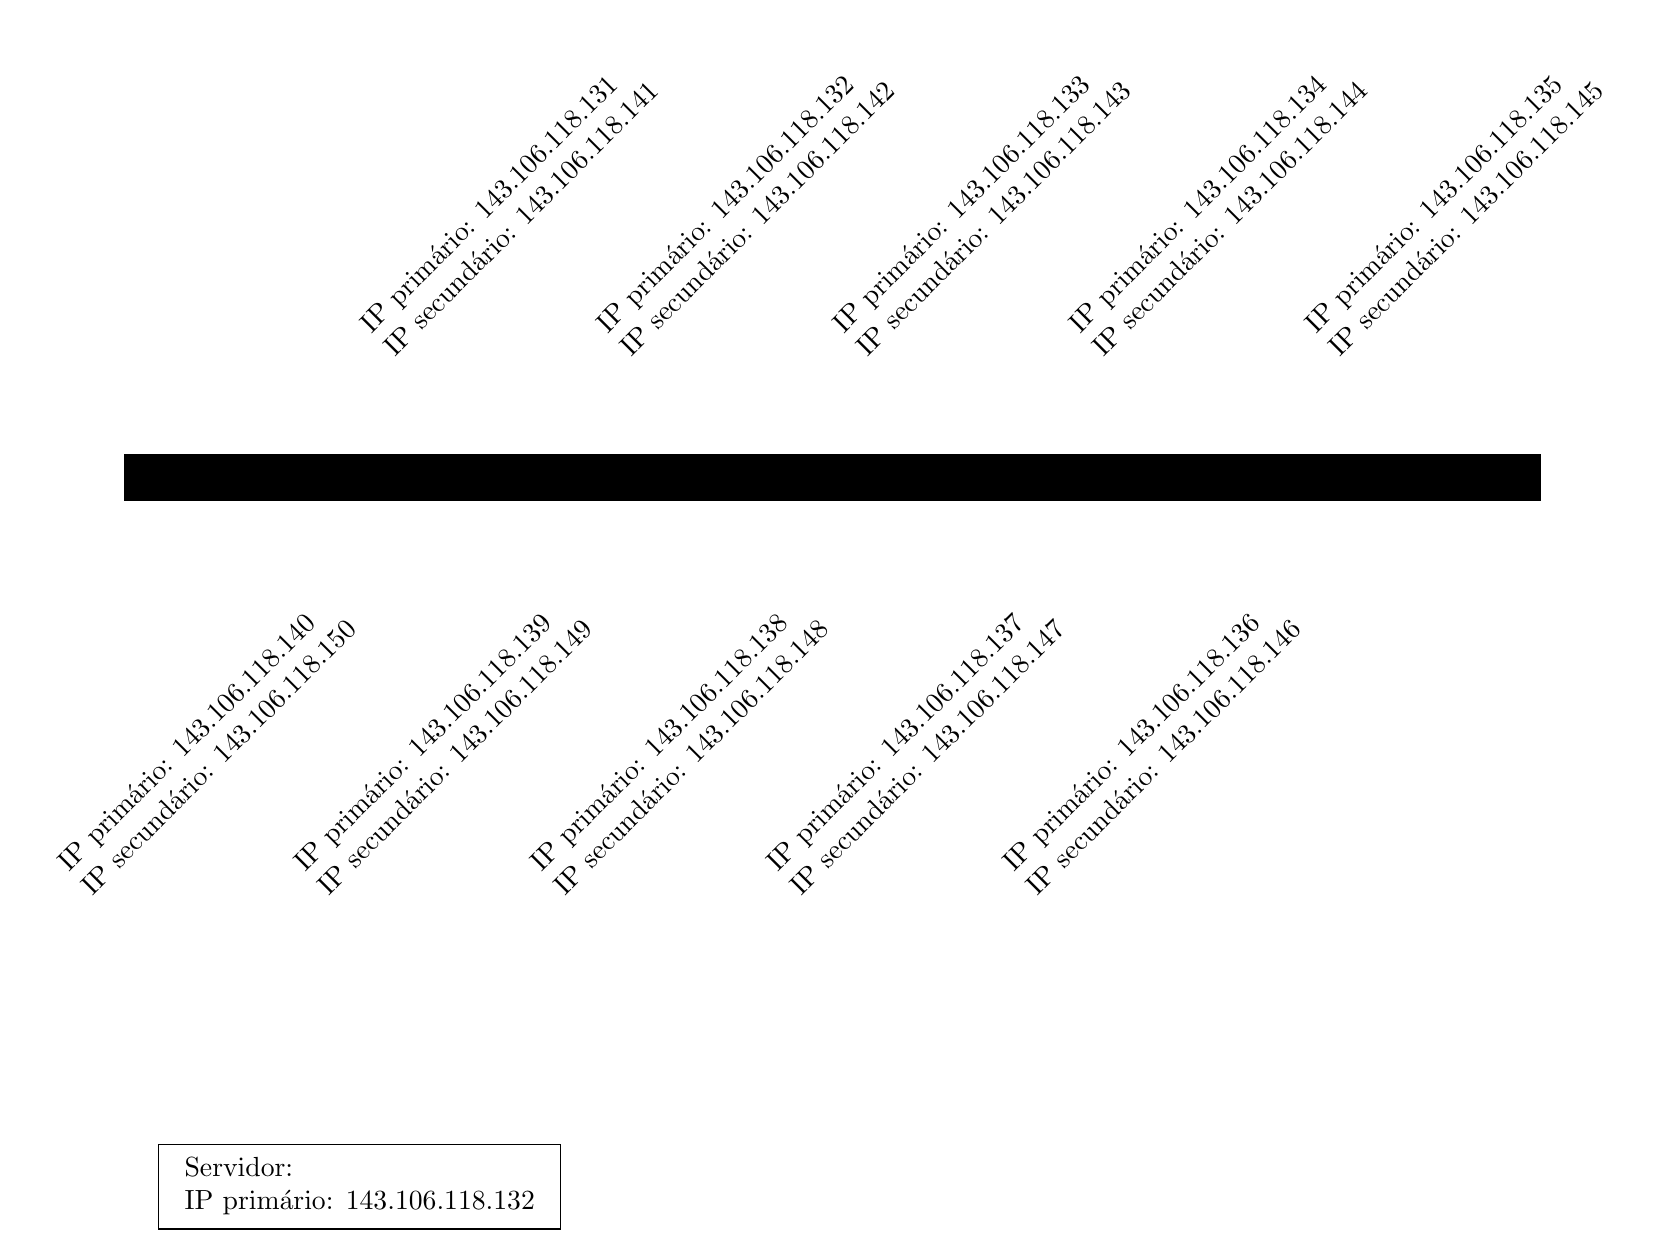
\begin{tikzpicture}[scale=3]
    \fill (0,.1) rectangle (6,-.1);
    \coordinate (a) at (1,.5);
    \coordinate (b) at (2,.5);
    \coordinate (c) at (3,.5);
    \coordinate (d) at (4,.5);
    \coordinate (e) at (5,.5);
    \coordinate (f) at (5,-.5);
    \coordinate (g) at (4,-.5);
    \coordinate (h) at (3,-.5);
    \coordinate (i) at (2,-.5);
    \coordinate (j) at (1,-.5);
    \node[rotate=45, anchor=west] at (a) {\ipspot{143.106.118.131}{143.106.118.141}};
    \node[rotate=45, anchor=west] at (b) {\ipspot{143.106.118.132}{143.106.118.142}};
    \node[rotate=45, anchor=west] at (c) {\ipspot{143.106.118.133}{143.106.118.143}};
    \node[rotate=45, anchor=west] at (d) {\ipspot{143.106.118.134}{143.106.118.144}};
    \node[rotate=45, anchor=west] at (e) {\ipspot{143.106.118.135}{143.106.118.145}};
    \node[rotate=45, anchor=east] at (f) {\ipspot{143.106.118.136}{143.106.118.146}};
    \node[rotate=45, anchor=east] at (g) {\ipspot{143.106.118.137}{143.106.118.147}};
    \node[rotate=45, anchor=east] at (h) {\ipspot{143.106.118.138}{143.106.118.148}};
    \node[rotate=45, anchor=east] at (i) {\ipspot{143.106.118.139}{143.106.118.149}};
    \node[rotate=45, anchor=east] at (j) {\ipspot{143.106.118.140}{143.106.118.150}};

    \node[draw] at (1,-3) {\servidor{143.106.118.132}};
  \end{tikzpicture}
\end{center}
Broadcast: 143.106.118.159 \\
Net mask: 255.255.255.224 \\
DNS primário: 143.106.22.2 \\
DNS secundário: 143.106.7.7
\end{document}
